%\documentclass[mathserif]{beamer}
\documentclass[handout]{beamer}
%\usetheme{Goettingen}
\usetheme{Warsaw}
%\usetheme{Singapore}
%\usetheme{Frankfurt}
%\usetheme{Copenhagen}
%\usetheme{Szeged}
%\usetheme{Montpellier}
%\usetheme{CambridgeUS}
%\usecolortheme{}
%\setbeamercovered{transparent}
\usepackage[english, activeacute]{babel}
\usepackage[utf8]{inputenc}
\usepackage{amsmath, amssymb}
\usepackage{dsfont}
\usepackage{graphics}
\usepackage{cases}
\usepackage{graphicx}
\usepackage{pgf}
\usepackage{epsfig}
\usepackage{amssymb}
\usepackage{multirow}	
\usepackage{amstext}
\usepackage[ruled,vlined,lined]{algorithm2e}
\usepackage{amsmath}
\usepackage{epic}
\usepackage{fontenc}
\usepackage{framed,color}
\usepackage{palatino, url, multicol}
\usepackage{listings}
%\algsetup{indent=2em}
\vspace{-0.5cm}
\title{Probability}
\vspace{-0.5cm}
\author[Felipe Bravo Márquez]{\footnotesize
%\author{\footnotesize  
 \textcolor[rgb]{0.00,0.00,1.00}{Felipe José Bravo Márquez}} 
\date{ \today }


\begin{document}
\begin{frame}
\titlepage


\end{frame}


%%%%%%%%%%%%%%%%%%%%%%%%%%%

\begin{frame}{Probability and Statistics}

\scriptsize{
\begin{itemize}
 \item Probability is the language of \textbf{uncertainty} that is also the basis for statistical inference \cite{poldrack2019statistical}. 

 \item It forms an important part of the foundation for statistics, because it provides us with the mathematical tools to describe uncertain events. 
 \item The study of probability arose in part due to interest in understanding games of chance, like cards or dice. 
 \item These games provide useful examples of many statistical concepts, because when we repeat these games the likelihood of different outcomes remains (mostly) the same.
\end{itemize}

\begin{figure}[h!]
	\centering
	
\includegraphics[scale=0.2]{pics/gambling.png}
\end{figure}


}

\end{frame}


\begin{frame}{Probability and Statistics}

\scriptsize{
\begin{itemize}
  \item The problem studied in probability is: given a data generating process, which are the properties of the outputs?
 \item The problem studied in statistical inference, data mining and machine learning is: given the outputs, what can we say about the process that generates the observed data? 
\end{itemize}

}
\begin{figure}[h!]
	\centering
	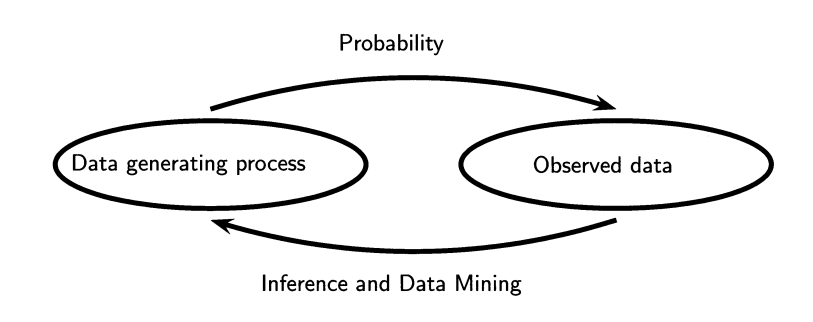
\includegraphics[scale=0.3]{pics/probandstats.png}
\end{figure}

\footnotemark{Figure taken from \cite{wasserman2013all}}

\end{frame}

\begin{frame}\frametitle{What is Probability?}
\scriptsize{

\begin{itemize}
 \item We think of probability as a number that describes the likelihood of some event occurring, which ranges from zero (impossibility) to one (certainty).
 \item Probabilities can also be expressed in percentages: when the weather forecast predicts a twenty percent chance of rain today. 
 \item In each case, these numbers are expressing how likely that particular event is, ranging from absolutely impossible to absolutely certain.
\end{itemize}

}

\end{frame}



\begin{frame}\frametitle{Probability Concepts}
\scriptsize{

\begin{itemize}
 \item A \textbf{random experiment} in the act of measuring a process whose output is uncertain. 
 \item Examples: flipping a coin, rolling a 6-sided die, or trying a new route to work to see if it’s faster than the old route.
 \item The set with all possible outputs of a random experiment is the \textbf{sample space} $\Omega$ (it can be discrete or continuous).
 \item For a coin flip  $\Omega = \{$heads, tails$\}$, for the 6-sided die  $\Omega = \{1,2,3,4,5,6\}$, and  for the amount of time it takes to get to work $\Omega$ is all possible real numbers greater than zero.
 \item An \textbf{event} $E \subseteq \Omega$ corresponds to a subset of those outputs.
 \item For example, $E = \{ 2,4,6 \}$ is the event of observing an even number when rolling a die.
\end{itemize}

}

\end{frame}

\begin{frame}\frametitle{Probability}
\begin{scriptsize}
\begin{itemize}
\item Now we can outline the formal features of a probability, which were first defined by the Russian mathematician Andrei Kolmogorov.
\begin{figure}[h!]
	\centering
	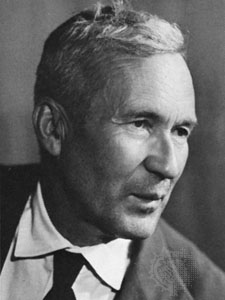
\includegraphics[scale=0.15]{pics/kolmogorov.jpeg}
\end{figure}



 \item A probability $\mathbb{P}$ is a real-valued function defined over $\Omega$ that satisfies the following properties:
\end{itemize}

\begin{block}{Properties}
\begin{enumerate}
 \item For any event $E \subseteq \Omega$ , $0 \leq \mathbb{P}(E) \leq 1$.
 \item The probability of the sample space is 1: $\mathbb{P}(\Omega) =1$
 \item Let $E_{1},E_{2},\dots,E_{k} \in \Omega$ be disjoint sets 
 \begin{displaymath}
  \mathbb{P}(\bigcup_{i=1}^{k}E_{i}) = \sum_{i}^{k}P(E_{i})
 \end{displaymath}
\end{enumerate}
\end{block}

Probabilities cannot be negative or greater than 1.

\end{scriptsize} 

\end{frame}


\begin{frame}\frametitle{Interpretation of Probabilities}
\begin{scriptsize}

The are two common interpretations of probabilities: frequencies and degrees of beliefs (or Bayesian probabilities).
\begin{block}{Frequentist probability}
\begin{itemize} 
 \item In the frequency interpretation, $\mathbb{P}(E)$ is the long run proportion (limiting frequency) of times that $E$ is true in repetitions.\footnote{\url{https://en.wikipedia.org/wiki/Frequentist_probability}} 
\item For example, if we say that the probability of heads is 1/2, we mean that if we flip the coin many times then the proportion of times we get heads tends to 1/2 as the number of tosses increases. 
\item When the sample space $\Omega$ is finite, we can say that
\begin{displaymath}
 \mathbb{P}(E) = \frac{\text{Favorable cases}}{\text{total cases}} = \frac{|E|}{|\Omega|}
 \end{displaymath}
\end{itemize} 
\end{block}



\end{scriptsize} 

\end{frame}



\begin{frame}\frametitle{Interpretation of Probabilities}
\begin{scriptsize}


\begin{block}{Probability as a degree of belief}
\begin{itemize} 
\item The degree-of-belief interpretation (a.k.a Bayesian interpretation or Subjective interpretation) is that $\mathbb{P}(E)$ measures an observer's strength of belief that $E$ is true.
\item If I were to ask you ``How likely is it that the US will return to the moon by 2026'', you can provide an answer to this question based on your knowledge and beliefs.
\item Even though there are no relevant frequencies to compute a frequentist probability.
\end{itemize}
\end{block}

\begin{itemize}
\item In either interpretation, we require that properties 1 to 3 hold.
\item The difference in interpretation will not matter much until we deal with statistical inference. 
\item There, the differing interpretations lead to two schools of inference: the frequentist and the Bayesian schools.
\end{itemize} 



\end{scriptsize} 

\end{frame}


\begin{frame}\frametitle{The rule of subtraction}
\scriptsize{

\begin{itemize}
 \item The probability of some event $E$ not happening is one minus the probability of the event happening:
 \begin{displaymath}
 \mathbb{P}(\neg E) = 1 - \mathbb{P}(E) 
 \end{displaymath}
\item For example, if the probability of rolling a one in a single die throw is 1/6, then the probability of rolling anything other than a one is 5/6.
 
\end{itemize}

}

\end{frame}


\begin{frame}\frametitle{Combinatorial methods}
\begin{scriptsize}


\begin{itemize} 
 \item There are a few facts from counting theory that are useful for calculating probabilities.
 \item Given $n$ objects, the number of ways of ordering these objects is $n!=n(n-1)(n-2)\cdots3\cdot2\cdot1$.
 \item For convenience, we define $0!=1$.
 \item We also define 
 \begin{displaymath}
  {n \choose k} = \frac{n!}{k!(n-k)!}
 \end{displaymath}
read ``n choose k'', which is the number of distinct ways of choosing k objects from n.
\end{itemize} 

\end{scriptsize} 

\end{frame}

\begin{frame}[fragile]\frametitle{Combinatorial methods}
\begin{scriptsize}


\begin{itemize} 
\item For example, if we have a class of 20 people and we want to select a committee of 3 students, then there are
 \begin{displaymath}
  {20 \choose 3} = \frac{20!}{3!17!}=1140
 \end{displaymath}
 possible committees.
 
\item In R:
 
 \begin{verbatim}
> factorial(20)/(factorial(3)*factorial(17))
[1] 1140
> choose(20,3)
[1] 1140  
 \end{verbatim}

 
 
 \item We note the following properties: 
 \begin{displaymath}
  {n \choose 0} = {n \choose n}=1
 \end{displaymath}
and
 \begin{displaymath}
  {n \choose k} = {n \choose n-k}.
 \end{displaymath}

\begin{verbatim}
> choose(20,17)
[1] 1140 
\end{verbatim}

 
 
\end{itemize} 
 
\end{scriptsize} 

\end{frame}


\begin{frame}{Conditional Probabilities}
\scriptsize{
\begin{itemize}
\item The \textbf{conditional probability} for $Y$ given $X$ is defined as:
 \begin{displaymath}
  \mathbb{P}(Y|X) = \frac{\mathbb{P}(X,Y)}{\mathbb{P}(X)}
 \end{displaymath}
 \item $\mathbb{P}(Y|X)$ can be interpreted as the fraction of times $Y$ occurs when $X$ is known to occur.
  \item  If $X$ and $Y$ are independent $\mathbb{P}(Y|X)=\mathbb{P}(Y)$
\end{itemize}

\begin{block}{Warning}
\begin{itemize}
 \item In general it is not the case that $\mathbb{P}(Y|X) = \mathbb{P}(X|Y)$. 
\item People get this confused all the time. 
\item For example, the probability of spots given you have measles is 1 but the probability that you have measles given that you have spots is not 1. 
\item In this case, the difference between $\mathbb{P}(Y|X)$ and $\mathbb{P}(X|Y)$ is obvious but there are cases where it is less obvious.
\end{itemize}
 
\end{block}



} 
\end{frame}



\begin{frame}[fragile]{Conditional Probabilities: Example}
\scriptsize{
\begin{itemize}
\item A medical test for a disease D has outcomes ``positive'' and ``negative'',  the probabilities are:

\begin{center}
\begin{tabular}{c|cc}
& D & $\neg$ D \\  \hline
positive & 0.009 & 0.099 \\
negative & 0.001 & 0.891 \\ 
\end{tabular}
\end{center}

\item From the definition of conditional probability

\begin{displaymath}
\mathbb{P}(\text{positive}|D) = \frac{\mathbb{P}(\text{positive},D)}{\mathbb{P}(D)}  = \frac{0.009}{0.009+0.001} = 0.9  
\end{displaymath}

\begin{verbatim}
> pos.d <- 0.009/(0.009+0.001)
> pos.d
[1] 0.9 
\end{verbatim}



and 
\begin{displaymath}
\mathbb{P}(\text{negative}|\neg D) = \frac{\mathbb{P}(\text{negative},\neg D)}{\mathbb{P}(\neg D)}  = \frac{0.891}{0.891+0.0991} \approx 0.9  
\end{displaymath}

\begin{verbatim}
> neg.notd <- 0.891/(0.891+0.0991)
> neg.notd
[1] 0.8999091 
\end{verbatim}



\end{itemize}




} 
\end{frame}


\begin{frame}[fragile]{Conditional Probabilities: Example}
\scriptsize{
\begin{itemize}
\item Apparently, the test is fairly accurate. 
\item Sick people yield a positive 90 percent of the time and healthy people yield a negative about 90 percent of the time.
\item Suppose you go for a test and get a positive. 
\item What is the probability you have the disease? Most people answer $0.90$. 
\item The correct answer is
\begin{displaymath}
\mathbb{P}(D|\text{positive}) = \frac{\mathbb{P}(D,\text{positive})}{\mathbb{P}(\text{positive})}  = \frac{0.009}{0.009+0.099} \approx 0.08  
\end{displaymath}
\begin{verbatim}
> d.pos <- 0.009/(0.009+0.099)
> d.pos
[1] 0.08333333 
\end{verbatim}



\item The lesson here is that you need to compute the answer numerically. 
\item Don't trust your intuition.
 
\end{itemize}




} 
\end{frame}




\begin{frame}{Bayes' Theorem and Total Probabilities}
\scriptsize{
\begin{itemize}
 \item The conditional probability $\mathbb{P}(Y|X)$ and $\mathbb{P}(X|Y)$ can be expressed as a function of each other using Bayes' theorem.
\begin{displaymath}
 \mathbb{P}(Y|X)=\frac{\mathbb{P}(X|Y)\mathbb{P}(Y)}{\mathbb{P}(X)}
\end{displaymath}
\item Then let $\{ Y_1,Y_2,\dots, Y_k \} $ be a set of mutually exclusive events of the sample space of a R.V $X$, the denominator of Bayes' theorem can be expressed as:
\begin{displaymath}
\mathbb{P}(X)= \sum_{i=1}^{k} \mathbb{P}(X,Y_i) = \sum_{i=1}^{k} \mathbb{P}(X|Y_i)\mathbb{P}(Y_i)
\end{displaymath}
\end{itemize}
 
}
\end{frame}

\begin{frame}{Example}
\scriptsize{
\begin{itemize}
 \item I split my emails into three categories: $A_1$=```spam'', $A_2$=```low priority'', $A_3$=```high priority''.'
 \item We know that $\mathbb{P}(A_1)=0.7$, $\mathbb{P}(A_2)=0.2$ and $\mathbb{P}(A_3)=0.1$, clearly $0.7+0.2+0.1=1$.
 \item Let $B$ be the event that the mail contains the word ``free''.
 \item We know that $\mathbb{P}(B|A_1)=0.9$ $\mathbb{P}(B|A_2)=0.01$ y $\mathbb{P}(B|A_3)=0.01$ clearly $0.9+0.01+0.01 \neq 1$
 \item  What is the probability that an email with the word ``free'' in it is ``spam''?
 \item Using Bayes:
 \begin{displaymath}
   \mathbb{P}(A_1|B) = \frac{\mathbb{P}(B|A_1)\times \mathbb{P}(A_1)}{\mathbb{P}(B)} = \frac{0.9 \times 0.7}{\mathbb{P}(B)} = \frac{0.63}{\mathbb{P}(B)}
 \end{displaymath}

 
\end{itemize}


} 
\end{frame}

\begin{frame}[fragile]{Example}
\scriptsize{
\begin{itemize}
 \item Using Total Probabilities:
 
  \begin{eqnarray*}
  \mathbb{P}(B) & = & \mathbb{P}(B|A_1)\times\mathbb{P}(A_1)+\mathbb{P}(B|A_2)\times\mathbb{P}(A_2)+\mathbb{P}(B|A_3)\times\mathbb{P}(A_3) \\
  & = & 0.9 \times 0.7 + 0.01 \times 0.2 + 0.01 \times 0.1 = 0.633
 \end{eqnarray*}

Finally =  


 
 
 \begin{displaymath}
  \mathbb{P}(A_1|B) = \frac{0.62}{0.633} = 0.995
 \end{displaymath}

\item In R:
\begin{verbatim}
> a1 <-0.7
> a2 <- 0.2
> a3 <-0.1
> b.a1 <- 0.9 
> b.a2<-0.01
> b.a3<-0.01
> b<-b.a1*a1+b.a2*a2+b.a3*a3
> a1.b<-b.a1*a1/b
> a1.b
[1] 0.9952607 
\end{verbatim}


\end{itemize}




} 
\end{frame}





\begin{frame}{Random Variable}
\scriptsize{

\begin{itemize}
 \item A \textbf{random variable} is a mapping (or function)
\begin{displaymath}
 X: \Omega \rightarrow \mathbb{R}
\end{displaymath}
which assigns a real value $X(e)$ to any event of $\Omega$.


\item Example: We flip a fair coin 10 times. The outcome of each toss is a head $H$ or a tail $T$.

\item  Let $X(e)$ be the number of heads in the sequence of outcomes.
\begin{itemize}
 \item If $e=HHTHHTHHTT$, then $X(e)=6$ 
\end{itemize}

\end{itemize}
}

\end{frame}


\begin{frame}{Random Variable}
\scriptsize{

\begin{itemize}
\item A random variable can in many cases be the identity function.

\item Example, if we roll a 6-sided die once and $X(e)$ is the resulting die value, then $X(e)=e$, for $e \in \{1,2,3,4,5,6\}$.

\item In these cases, the notion that a random variable is a function can be confusing (it looks more like a set), but we can always reconstruct the mapping function as the identity function.  

\item  It is important to understand that we can easily have different random variables from a same sample space. 

\item Example: we roll a die two times, $X(e)$ is the sum of the resulting two rolls and $Y(e)$ is the product of these two numbers.

\item For the event $e=\{4,5\}$, $X(e)=9$ and $Y(e)=45$.

\end{itemize}
}




\end{frame}



\begin{frame}{Example}

\begin{itemize}
 \item We flip a fair coin 2 times. Let $X$ be the number of heads obtained.
 \item The random variable and its distribution is summarized as:
\end{itemize}

\begin{table}
\begin{tabular}{c c|c}
\hline
 $e$ & $\mathbb{P}(e)$ & $X(e)$   \\ 
\hline
TT & 1/4 & 0 \\
TH & 1/4 & 1 \\
HT & 1/4 & 1 \\
HH & 1/4 & 2 \\
\hline
\end{tabular}
\end{table}

\begin{table}
\begin{tabular}{c|c}
\hline
 $x$ & $\mathbb{P}(X = x)$   \\ 
\hline
0 & 1/4 \\
1 & 1/2  \\
2 & 1/4  \\
\hline
\end{tabular}
\end{table}

\end{frame}




\begin{frame}{R.V Definitions}
\scriptsize{
\begin{itemize}
 \item  Let $X$ be a R.V , we define \textbf{cumulative distribution function} (CDF) or $F_{X}: \mathbb{R} \rightarrow [0,1]$ as:
\begin{displaymath}
 F_{X}(x)=\mathbb{P}(X\leq x)
\end{displaymath}
\item For the previous example of flipping a fair coin twice and counting the number of heads, the CDF is as follows:

\[   
F_X(x) = 
     \begin{cases}
     0 & x<0 \\
     1/4 & 0 \leq x < 1 \\
     3/4 & 1 \leq x < 2 \\
     1 & x \geq 2.
     \end{cases}
\]



\end{itemize}


} 
\end{frame}




\begin{frame}{R.V Definitions}
\scriptsize{

\begin{figure}[h!]
	\centering
	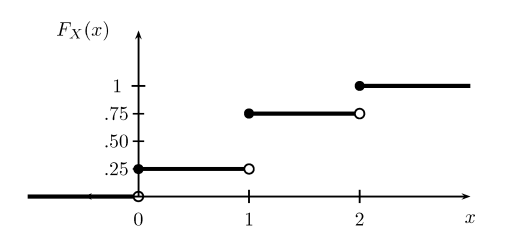
\includegraphics[scale=0.4]{pics/cdf_coin.png}
\end{figure}


\begin{itemize}
 \item CDF's can be very confusing. 
 \item Notice that the function is right continuous, non-decreasing, and that it is defined for all x, even though the random variable only takes values 0,1, and 2.
 \item Notation: when $X$ is a random variable; $x$ denotes a particular value of the random variable.
 
\end{itemize}


} 
\end{frame}


\begin{frame}{R.V Definitions}
\scriptsize{

\begin{block}{Discrete Random Variables}
\begin{itemize}
\item A R.V $X$ is \textbf{discrete} if it maps the outputs to a countable set.
\item We define the \textbf{probability function} or \textbf{probability mass function} PMF of a discrete R.V $X$ as $f_{X}(x)=\mathbb{P}(X=x)$.
\item Then $f_{X}(x) \geq 0$  $\forall x \in \mathbb{R}$, and $\sum_{i}f_{X}(x_{i})=1$
\item The CDF of $X$ is related to $f_{X}$ as follows: 
\begin{displaymath}
F_{X}= \mathbb{P}(X\leq x)= \sum_{x_{i} \leq x} f_{X}(x_{i})  
\end{displaymath}
  
\end{itemize}
 
\end{block}
The PMF for the previous example is:

\[   
f_X(x) = 
     \begin{cases}
     1/4 & x=0 \\
     1/2 & x=1 \\
     1/4 & x=2 \\
     0 &  \text{otherwise.}
     \end{cases}
\]


} 
\end{frame}



\begin{frame}{R.V Definitions}
\scriptsize{
\begin{block}{Continuous Random Variable}
\begin{itemize}
 \item A R.V $X$ is continuous if:
 \item there exists a function  $f_{X}$ such that $f_{X}(x) \geq 0$ $\forall x$,  $\int_{-\infty}^{\infty}f_{X}(x)dX=1$
 \begin{displaymath}
      \int_{-\infty}^{\infty}f_{X}(x)dX=1
       \end{displaymath}
\item For all $a \geq b$:
\begin{displaymath}
 \mathbb{P}(a < X < b) = \int_{a}^{b} f_{X}(x)dx
\end{displaymath}
\end{itemize}

\end{block}

\begin{itemize}
 \item The function $f_{X}$ is called the probability density function (PDF). 
 \item The PDF is related to the CDF as follows:
 \begin{displaymath}
 F_{X}(x)=\int_{-\infty}^{x}f_{X}(t)dt 
 \end{displaymath}
\item Then $f_{X}(x) = F'_X(x)$ at all points $x$ where $F_{X}$ is differentiable.
\end{itemize}

}
\end{frame}

\begin{frame}{R.V Definitions}
\scriptsize{
\begin{itemize}
 \item Example: Suppose that $X$ has PDF
 \[   
f_X(x) = 
     \begin{cases}
     1 & \text{for }0\leq x \leq 1 \\
     0 &  \text{otherwise.}
     \end{cases}
\]
 
\item Clearly, $f_X(x) \geq 0$ and $\int f_X(x) = 1$. 
\item A random variable with this density is said to have a Uniform (0,1) distribution.
\item This is meant to capture the idea of choosing a point at random between 0 and 1. 
\item The CDF is given by 
 \[   
F_X(x) = 
     \begin{cases}
     0 & x<0 \\
     x &  0\leq x \leq 1 \\
     1 &  x>1. 
     \end{cases}
\] 
 
\begin{figure}[h!]
	\centering
	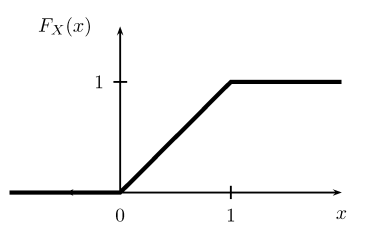
\includegraphics[scale=0.4]{pics/cdf_uniform.png}
\end{figure} 
 
\end{itemize}




}
\end{frame}


\begin{frame}{R.V Definitions}
\scriptsize{
\begin{itemize}
 \item Continuous random variables can lead to confusion. 
 \item First, note that if $X$ is continuous then $\mathbb{P}(X = x) = 0$ for every $x$. 
\item Don't try to think of $f(x)$ as $\mathbb{P}(X = x)$. 
\item This only holds for discrete random variables. 
\item We get probabilities from a PDF by integrating. 

\end{itemize}




}
\end{frame}


\begin{frame}{R.V Definitions}
\scriptsize{
\begin{itemize}
\item A PDF can be bigger than 1 (unlike a mass function). 
\item For example, if $f(x) = 5$ for $x \in  [0,1/5]$ and $0$ otherwise.
\item Then $f(x) \geq 0$ and $\int f(x)dx = 1$, so this is a well-defined PDF even though $f(x) = 5$ in some places.
\item A PDF can also be interpreted as the rate of change in the CDF. 
\item So where cumulative probability is increasing rapidly, density can easily exceed 1. 
\item But if we calculate the area under the density function, it will never exceed 1. 
 
\end{itemize}




}
\end{frame}


\begin{frame}{Some Properties}

\begin{enumerate}
 \item $ \mathbb{P}( x < X \leq y) = F(y) - F(x)$
       

\item $ \mathbb{P}(X > x) = 1 - F(x)$ 

\item If $X$ is continuous: 
\begin{eqnarray*}
 F(b) - F(a) = \mathbb{P}(a < X < b) = \mathbb{P} ( a \leq X < b)  \\
   = \mathbb{P} ( a < X \leq b) = \mathbb{P} ( a \leq X \leq b) 
\end{eqnarray*}

\end{enumerate}



 
\end{frame}



\begin{frame}{Quantiles}
\scriptsize{
\begin{itemize}
 \item Let $X$ be a R.V with CDF $F$. The inverse CDF or quantile function is defined as \begin{displaymath}
                                                                                   F^{-1}(q)= inf \left\{ x: \ F(x) > q \right\}
                                                                                     \end{displaymath}
 \item For $q \in [0,1]$ if $F$ is strictly increasing and continuous, $F^{-1}(q)$ is the only real value such that $F(x)=q$.
 \item Then $F^{-1}(1/4)$ is the first quartile, $F^{-1}(1/2)$ the median (or second quartile) and $F^{-1}(3/4)$ the third quartile.
 
 
\end{itemize}

}

\end{frame}




\begin{frame}{Some distributions}
\scriptsize{ 

\begin{table}
\centering
\begin{tabular}{c|c|c}
\hline
  & Probability Function & Parameters   \\ 
\hline
Binomial & $f_x= {n \choose x}p^{x}(1-p)^{n-x} $ & $n,p$ \\ \hline
Normal & $f_x=\frac{1}{\sqrt{2\pi}\sigma}\exp^{-\frac{1}{2}\frac{(x-\mu)^2}{\sigma^{2}}}$ & $\mu, \sigma$ \\ \hline
Poisson & $f_x=\frac{1}{x!}\lambda^{x}\exp^{-\lambda}$ & $\lambda$ \\ \hline
Exponential & $f_x= \lambda \exp^{-\lambda x}$  & $\lambda$ \\ \hline
Gamma & $f_x= \frac{\lambda^{\alpha}}{\Gamma(\alpha)} x^{\alpha -1}\exp^{-\lambda x} $ & $\lambda , \alpha$ \\ \hline
Chi-square & $f_x=\frac{1}{2^{k/2} \Gamma(k/2)} x^{(\frac{k}{2} -1)} \exp^{-x/2} $  & $k$  \\
\hline
\end{tabular}
\end{table}

\begin{block}{Warning}
We defined random variables to be mappings from a sample space $\Omega$ to $\mathbb{R}$ but we did not mention the sample space in any of the distributions above. The sample space often becomes implicit but it is really there in the background. 
\end{block}



}
\end{frame}



\begin{frame}[fragile]{Binomial Distribution}

\scriptsize{
\begin{itemize}
 \item  The binomial distribution is a discrete distribution that provides a way to compute the probability of some number of successes out of a number of trials.
 \item In each trial there is either success or failure and nothing in between (known as “Bernoulli trials”) given some known probability of success on each trial.
 \item Let $n$ be the number of trials, $x$ the number of successes, and $p$ the probability of a success, the probability mass function of the Binomial distribution is as follows:
 \begin{displaymath}
  f_x(n,p)= {n \choose x}p^{x}(1-p)^{n-x} 
 \end{displaymath}
\item The binomial coefficient ${n \choose x}$ describes the number of different ways that one can choose $x$ items out of $n$ total items.

 \end{itemize}}
 
 \end{frame}
 
 
\begin{frame}[fragile]{Binomial Distribution}

\scriptsize{
\begin{itemize}
\item Example: on Jan 20 2018, the basketball player Steph Curry hit only 2 out of 4 free throws in a game against the Houston Rockets.
\item We know that Curry's overall probability of hitting free throws across the entire season was 0.91.
\item What is probability that he would hit only 50\% of his free throws in a game?
\begin{displaymath}
 f_2(4,0.91) = {4 \choose 2}0.91^{2}(1-0.91)^{4-2}=0.040 
\end{displaymath}
In R: 
\begin{verbatim}
> choose(4,2)*0.91^2*(1-0.91)^2
[1] 0.04024566
> # more compactly
> dbinom(x=2,size=4,p=0.91)
[1] 0.04024566
\end{verbatim}
 
 \end{itemize}}
 
 \end{frame}


 

\begin{frame}{The Normal Distribution}

\scriptsize{
\begin{itemize}
 \item  The normal or Gaussian distribution is extremely important in statistics, in part because it shows up all the time in nature. 
 \item It is controlled by two parameters, a mean $\mu$ and a standard deviation $\sigma$. 
 
 \begin{figure}[h!]
	\centering
	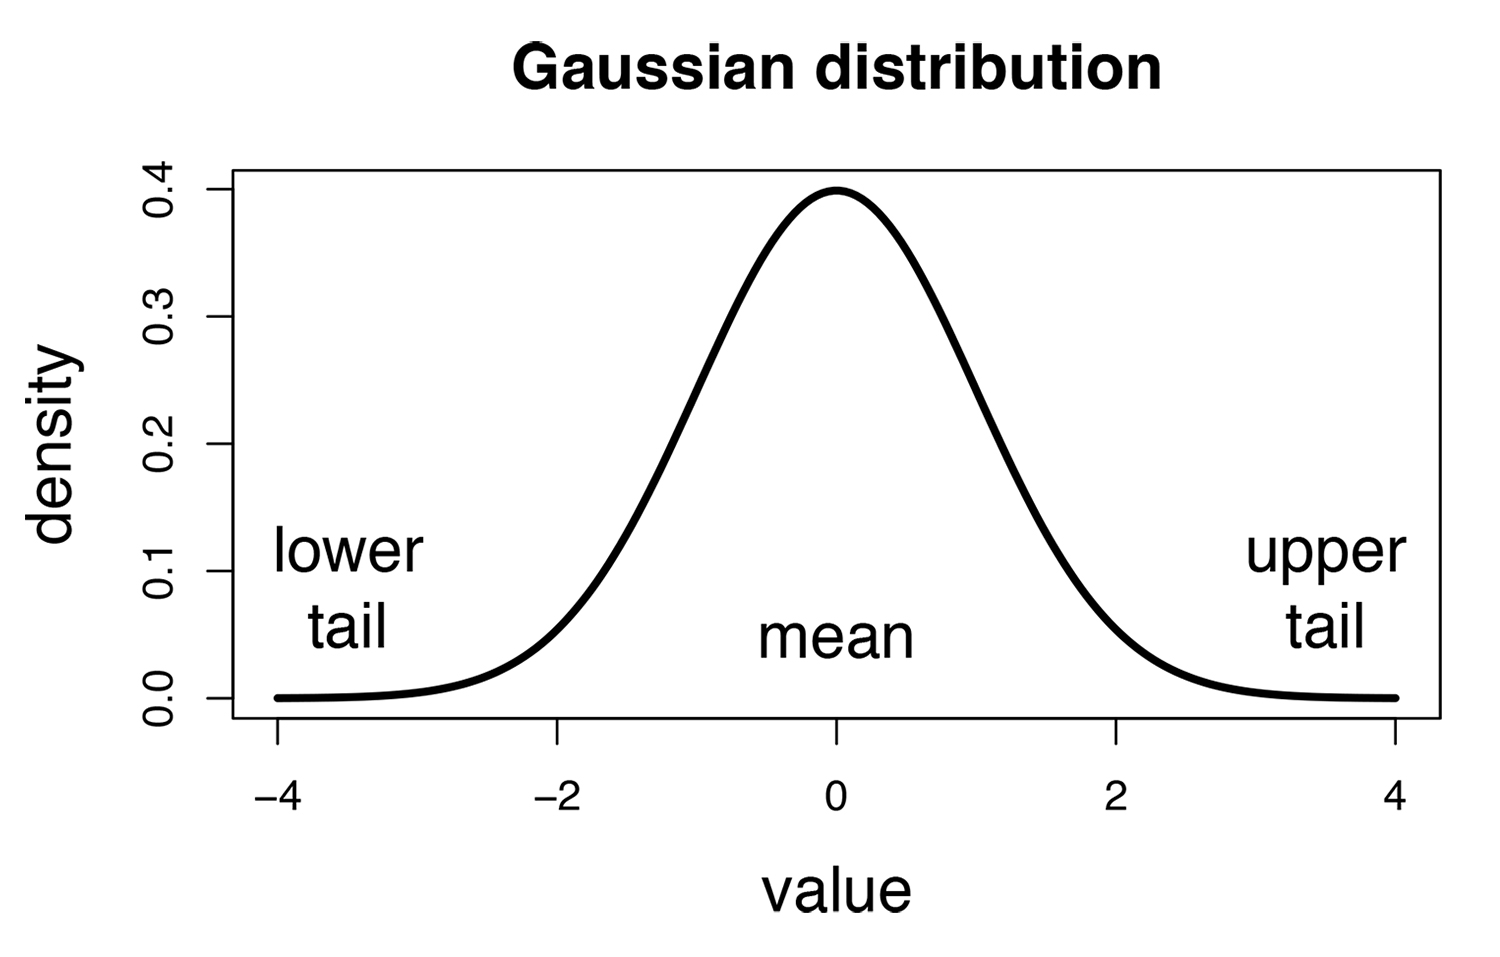
\includegraphics[scale=0.13]{pics/gaussian.jpg}
\end{figure}
 
 \item As we will see in the following example~\cite{mcelreath2020statistical}, the normal distribution is observed whenever many small, independent variations are summed together to produce a value.
 \end{itemize}}
 
 \footnotemark{Figure source: \url{http://sfonline.barnard.edu/wp-content/uploads/2015/12/gaussian-distribution.jpg}}
 
 \end{frame}



\begin{frame}{Normal Distribution}

\scriptsize{
\begin{itemize}
 \item  Suppose you and a thousand of your closest friends line up on the halfway line of a soccer field (football pitch).
 \item Each of you has a coin in your hand. At the sound of the whistle, you begin flipping the coins. 
 \item Each time a coin comes up heads, that person moves one step
towards the left-hand goal. 
\item Each time a coin comes up tails, that person moves one step towards the right-hand goal. 
\item Each person flips the coin 16 times, follows the implied moves,
and then stands still.
\item Now we measure the distance of each person from the halfway line.
\item Can you predict what proportion of the thousand people who are standing on the halfway line? How about the proportion 5 yards left of the line?
 \end{itemize}}
 
 \end{frame}
 
\begin{frame}{Normal Distribution}

\scriptsize{
\begin{itemize}
\item It’s hard to say where any individual person will end up, but you can say with great confidence what the collection of positions will be. 
\item The distances will be distributed in approximately normal, or Gaussian, fashion.
\item This is true even though the underlying distribution is binomial. 
\item It does this because there are so many more possible ways to realize a sequence of left-right steps that sums to zero. 
\item There are slightly fewer ways to realize a sequence that ends
up one step left or right of zero, and so on, with the number of possible sequences declining in the characteristic bell curve of the normal distribution.
 \end{itemize}}
 
 \end{frame}
 



\begin{frame}{Soccer 1}
 \begin{figure}[h!]
	\centering
	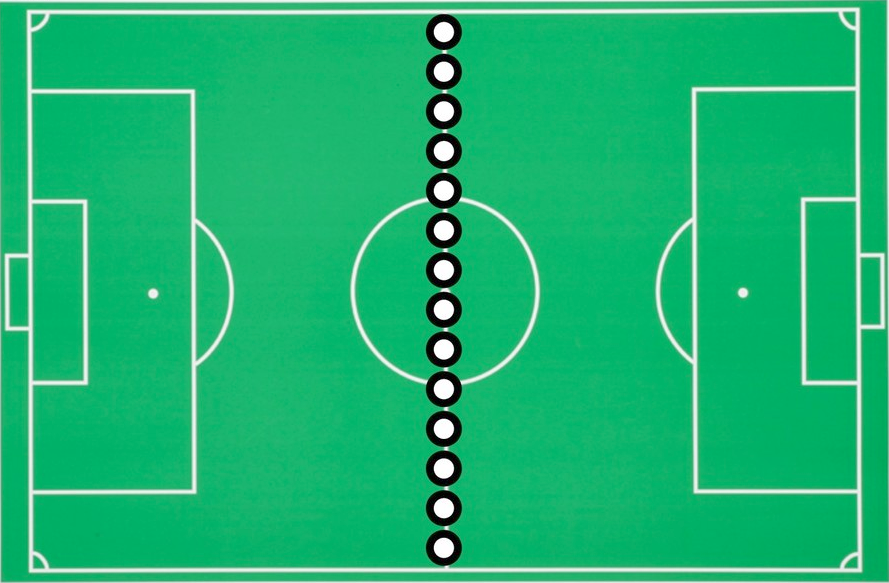
\includegraphics[scale=0.3]{pics/soccer1.png}
	\caption{Source: \url{https://github.com/rmcelreath/stat_rethinking_2020}}
\end{figure}


\end{frame}


\begin{frame}{Soccer 2}
 \begin{figure}[h!]
	\centering
	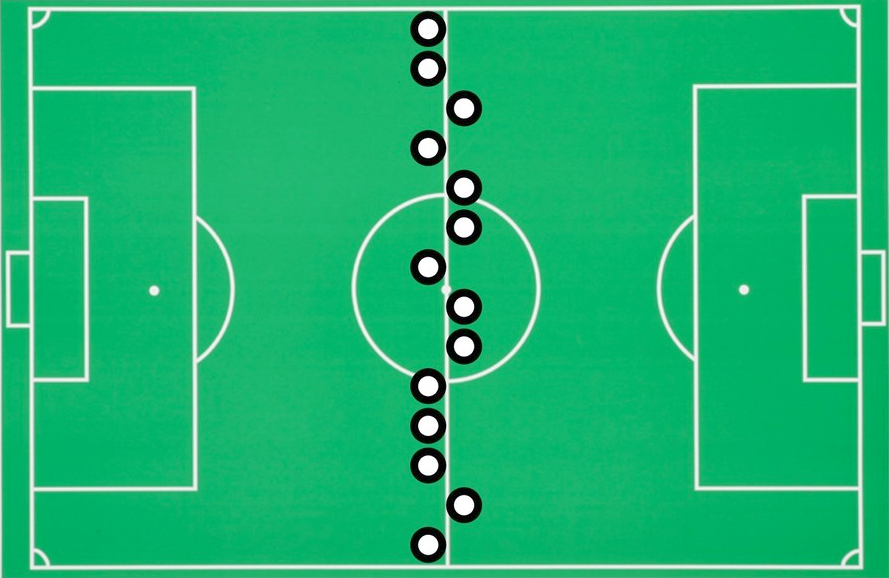
\includegraphics[scale=0.3]{pics/soccer2.png}
\end{figure}


\end{frame}

\begin{frame}{Soccer 3}
 \begin{figure}[h!]
	\centering
	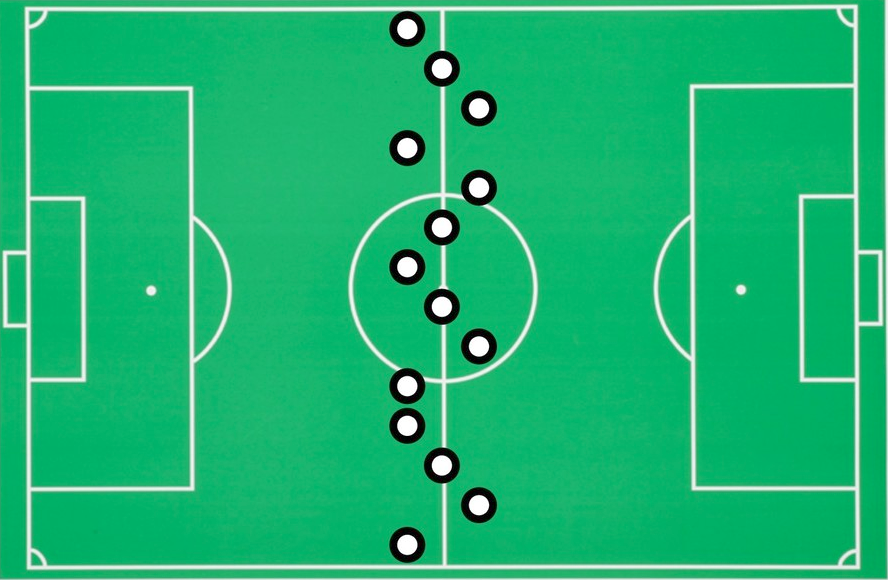
\includegraphics[scale=0.3]{pics/soccer3.png}
\end{figure}


\end{frame}


\begin{frame}{Soccer 4}
 \begin{figure}[h!]
	\centering
	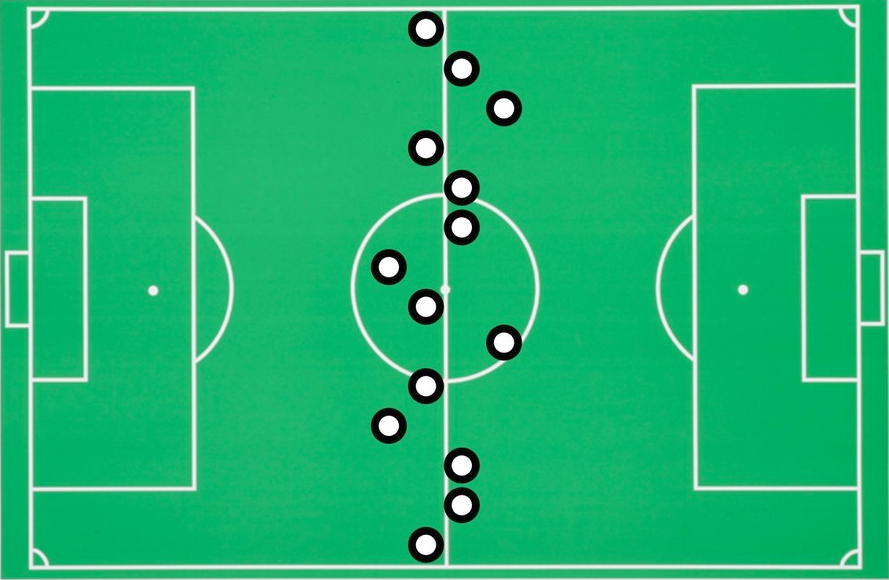
\includegraphics[scale=0.3]{pics/soccer4.png}
\end{figure}
\end{frame}


\begin{frame}{Soccer 5}
 \begin{figure}[h!]
	\centering
	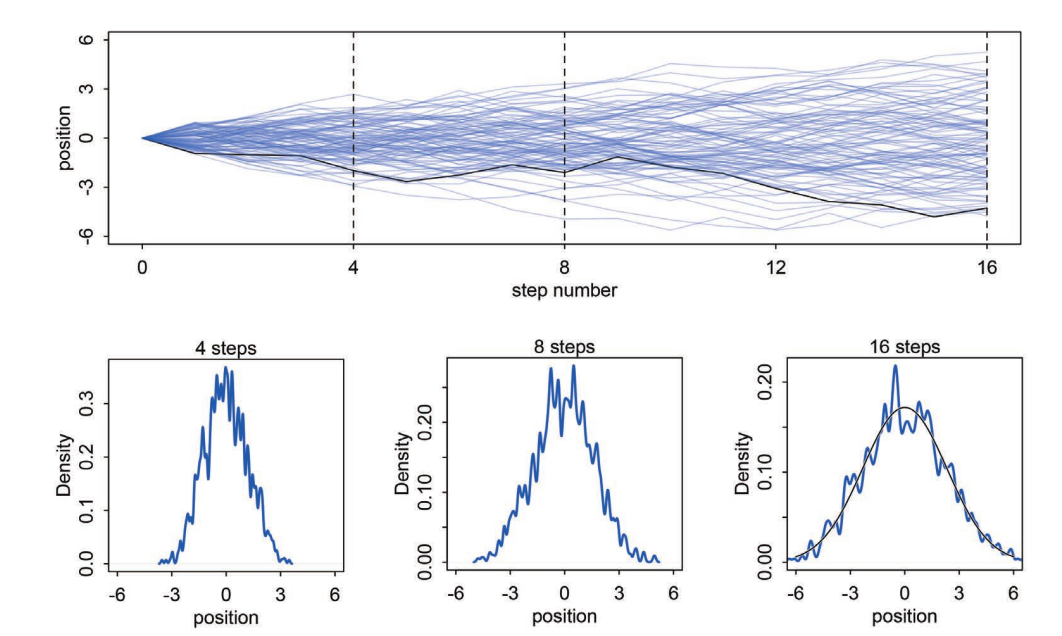
\includegraphics[scale=0.25]{pics/soccer5.png}
\end{figure}

\begin{scriptsize}
\begin{itemize}
 \item  Random walks on the soccer field converge to a normal distribution. 
 \item The more steps are taken, the closer the match between the real empirical distribution of positions and the ideal normal distribution, superimposed in the last plot in the bottom panel.
\end{itemize}
\end{scriptsize}

\end{frame}


\begin{frame}{The Normal Distribution}

\scriptsize{
\begin{itemize}
 \item $X$ has a Normal or Gaussian distribution of parameters $\mu$ and $\sigma$, $X \sim N(\mu,\sigma^2)$ if  
 \begin{displaymath}
 f_x=\frac{1}{\sqrt{2\pi}\sigma}\exp^{-\frac{1}{2}\frac{(x-\mu)^2}{\sigma^{2}}} 
 \end{displaymath}
 \item Where $\mu \in \mathbb{R}$ is the ``center'' or the ``mean'' of the distribution and $\sigma > 0$ is the ``standard deviation''.
 \item The mean shifts the distribution along the x axis. 
 \item The standard deviation affects the shape such that the larger the $\sigma$, the wider the shape.
 
 \item When $\mu = 0$ and $\sigma =1$ we have a \textbf{Standard Normal Distribution} denoted by $Z$.
 \item We refer to the PDF by $\phi(z)$ and to the CDF of a Standard Normal by $\Phi(z)$.
 
 \item The values of $\Phi(z)= \mathbb{P}(Z \leq z)$ are tabulated.
 
    
 \end{itemize}
}
\end{frame}



\begin{frame}{The Normal Distribution}


  \begin{figure}[h!]
	\centering
	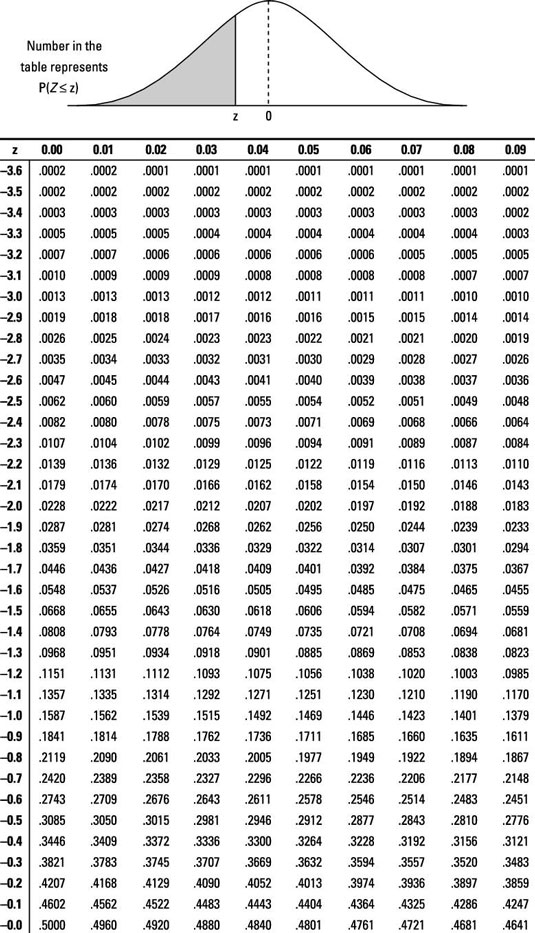
\includegraphics[scale=0.4]{pics/gaussianTable.jpg}
\end{figure}
 

\end{frame}




\begin{frame}{The Normal Distribution}

\scriptsize{
\begin{itemize}
 \item Let's try to understand the main components of $\phi(z)$ as showed in \cite{colin2020}.
 
  \begin{displaymath}
  \phi(z) = \frac{1}{\sqrt{2\pi}} \exp^{-\frac{1}{2}x^2}
 \end{displaymath}
 
 \item Here's a plot of just the exponent $-\frac{1}{2}x^2$.
 
  \begin{figure}[h!]
	\centering
	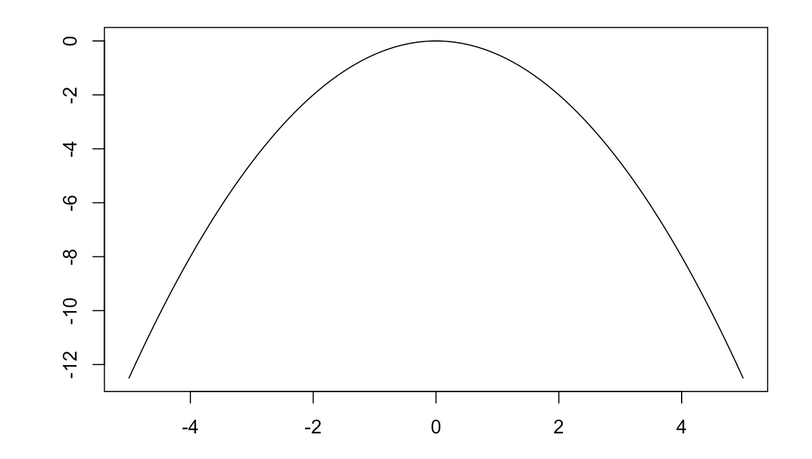
\includegraphics[scale=0.2]{pics/gauss_exp.png}
\end{figure}
 
 \item As you can see, this is a simple parabola. 

 \end{itemize}

}
\end{frame}



\begin{frame}{The Normal Distribution}

\scriptsize{
\begin{itemize}
 \item When we raise $\exp$ to the power of $-\frac{1}{2}x^2$ we get the following plot.
 
   \begin{figure}[h!]
	\centering
	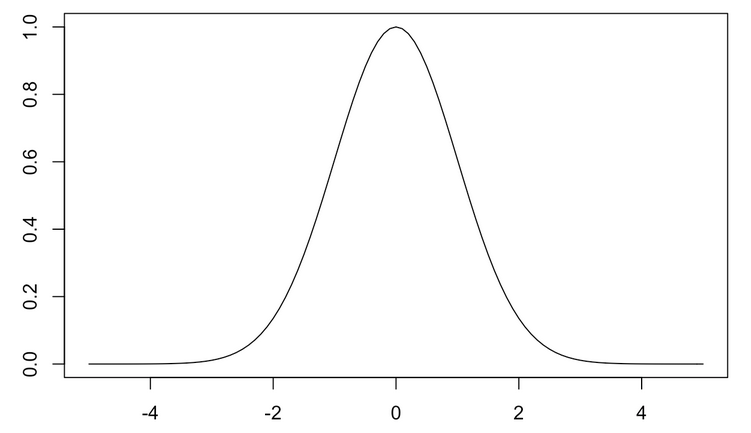
\includegraphics[scale=0.2]{pics/gauss_exp2.png}
\end{figure}
 
 \item Taking the exponential of a negative parabola is what gives us the bell curve. 
 \item As is, the area under the curve is $\sqrt{2\pi}$, so the constant $\frac{1}{\sqrt{2\pi}}$ is included to make it equal to 1.
 \item Finally, the $\frac{1}{2}$ in the exponent ensures that the variance is equal to 1. 
 \end{itemize}

}
\end{frame}

\begin{frame}{The  Normal Distribution}

\scriptsize{
\begin{itemize}
 \item In order to generalize to any normal distribution we simply include the parameters $\mu$ and $\sigma$
 \begin{displaymath}
 \frac{1}{\sqrt{2\pi}\sigma}\exp^{-\frac{1}{2}\frac{(x-\mu)^2}{\sigma^{2}}} 
 \end{displaymath}
 \item Notice that $\sigma$ scales the constant, but that the real action happens in the exponent. 
 \item The density's highest point is shifted by $\mu$, then divided by $\sigma$. 
\end{itemize}

\begin{block}{Useful Properties}
\begin{enumerate}
 \item If $X \sim N(\mu, \sigma^2)$, then $Z=(X-\mu)/\sigma \sim N(0,1)$.\footnote{This value is also called \textbf{Z-score}.}
 \item If $Z \sim N(0,1)$, then $X=\mu+\sigma Z \sim N(\mu, \sigma^2)$
 \item Let $X_{i} \sim N(\mu_{i},\sigma_{i}^{2})$ ,$i=1,\dots,n$ \  be independent R.Vs:
 \begin{displaymath}
  \sum_{i=1}^{n}X_{i}\sim N( \sum_{i=1}^{n}\mu_{i}, \sum_{i=1}^{n}\sigma_{i}^{2})
 \end{displaymath}

 
\end{enumerate}
 
\end{block}
}
\end{frame}



\begin{frame}{The  Normal Distribution}

\scriptsize{
\begin{itemize}
 \item If follows from property 1 that if $X\sim N(\mu,\sigma^2)$, then
 
 \begin{align}
  \mathbb{P}(a<X<b) & = \mathbb{P}\left(\frac{a-\mu}{\sigma}<X<\frac{b-\mu}{\sigma}\right) \\
   & = \Phi \left(\frac{b-\mu}{\sigma}\right)-\Phi \left(\frac{a-\mu}{\sigma}\right)
 \end{align}

 
\end{itemize}


}
\end{frame}




\begin{frame}{The Normal Distribution’s CDF}

\scriptsize{
\begin{itemize}
 \item As discussed above, when dealing with probability over continuous values we are primarily interested in probability over a range.
 \item For some purposes, it is convenient to think of a distribution in terms of total probability of an event occurring in the range of $-\infty$ to z.
 \item  For the standard normal distribution we get the following CDF:
 \begin{displaymath}
  \Phi(z)= \mathbb{P}(Z \leq z) = \frac{1}{\sqrt{2\pi}}\int_{-\infty}^{z} \exp^{\frac{-t^2}{2}}dt 
 \end{displaymath}
\item Here is a plot of the standard normal CDF.

   \begin{figure}[h!]
	\centering
	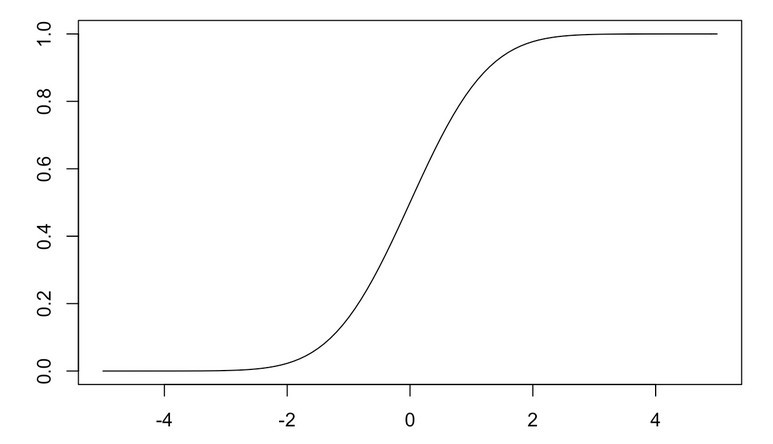
\includegraphics[scale=0.25]{pics/normalcdf.png}
\end{figure}
 
 \end{itemize}

}
\end{frame}


\begin{frame}{The Normal Distribution’s CDF}

\scriptsize{
\begin{itemize}
\item The y axis shows cumulative probability so  the function is always increasing.
 
\item The CDF is simply expressing the area under the curve (i.e. the integral from $-\infty$ to $z$) of the PDF. 
 
\item With $z = 0$, we are at the mean of the standard normal, so values are equally likely to be less than or greater than $z$. 

\item This means that the CDF at $z = 0$ should be $0.5$ as we have accumulated half of the available probability. 

   \begin{figure}[h!]
	\centering
	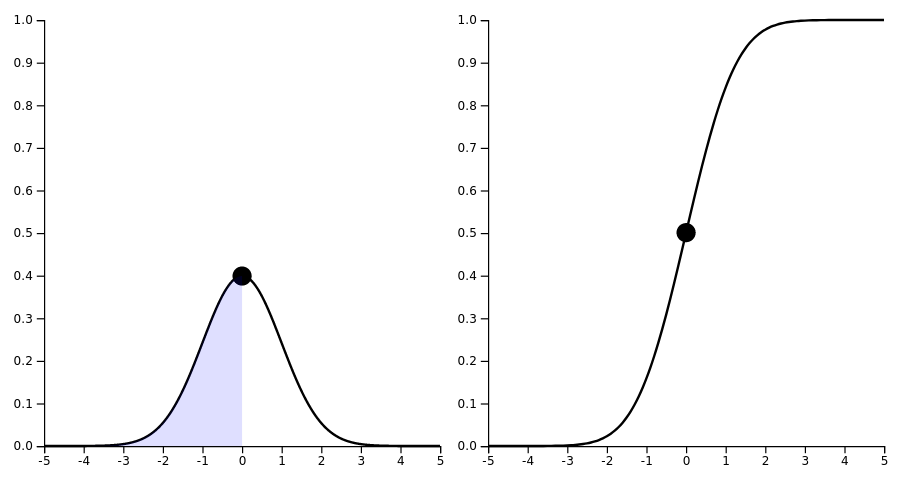
\includegraphics[scale=0.25]{pics/cdfpdf.png}
\end{figure}

 
 \end{itemize}

}
\end{frame}


\begin{frame}[fragile]{Example Normal}
\scriptsize{
\begin{itemize}
 \item In R we can access the PDF, CDF, quantile function and random number generation of the distributions.
 \item For a Normal distribution the R commands are:
\begin{verbatim}
dnorm(x, mean = 0, sd = 1, log = FALSE)
pnorm(q, mean = 0, sd = 1, lower.tail = TRUE, log.p = FALSE)
qnorm(p, mean = 0, sd = 1, lower.tail = TRUE, log.p = FALSE)
rnorm(n, mean = 0, sd = 1) 
\end{verbatim}
 
\end{itemize}

\begin{block}{Example}
Let $X\sim N(3,5)$, calculate $\mathbb{P}(X > 1)$ \\
$\mathbb{P}(X >1) = 1-\mathbb{P}(X<1) = 1-\mathbb{P}(Z < \frac{1-3}{\sqrt{5}})=1-\Phi(-0.8944)= 0.81$ \\
In R:
\begin{verbatim}
 > 1-pnorm(q=(1-3)/sqrt(5))
[1] 0.8144533
\end{verbatim}
Or directly:
\begin{verbatim}
> 1-pnorm(q=1,mean=3,sd=sqrt(5))
[1] 0.8144533 
\end{verbatim}
\end{block}
}
\end{frame}


\begin{frame}[fragile]{The 68-95-99.7 rule of a Normal Distribution}
\scriptsize{
\begin{figure}[h!]
	\centering
	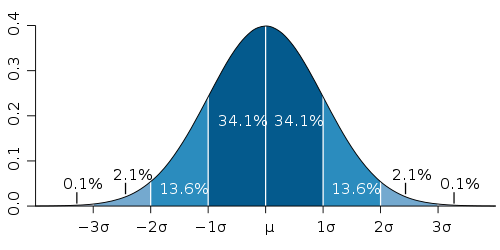
\includegraphics[scale=0.3]{pics/gaussian.png}
\end{figure} 
Let $X$ be a R.V $\sim N(\mu,\sigma^2)$.
\begin{itemize}
 \item $\mathbb{P}( \mu - \sigma \leq X \leq \mu+ \sigma) \approx 0.6827$  
 \item $\mathbb{P}( \mu - 2 \sigma \leq X \leq \mu+ 2 \sigma) \approx 0.9545$               
 \item $\mathbb{P}( \mu - 3 \sigma \leq X \leq \mu+ 3 \sigma) \approx 0.9973$ 

\end{itemize}
In R for $X\sim N(0,1)$:
\begin{verbatim}
> pnorm(1)-pnorm(-1)
[1] 0.6826895
> pnorm(2)-pnorm(-2)
[1] 0.9544997
> pnorm(3)-pnorm(-3)
[1] 0.9973002 
\end{verbatim}
}
\end{frame}

\begin{frame}[fragile]{Symmetry of the Normal Distribution}
\begin{itemize}
 \item The PDF of a normal is symmetric around $\mu$.
 \item Then $\phi(z)= \phi(-z) $ 
 \item $\Phi(z)=1-\Phi(-z)$
\end{itemize}
\begin{verbatim}
> dnorm(1)
[1] 0.2419707
> dnorm(-1)
[1] 0.2419707
> pnorm(0.95)
[1] 0.8289439
> 1-pnorm(-0.95)
[1] 0.8289439 
\end{verbatim}


\end{frame}

\begin{frame}[fragile]{Plotting the PDF of Normals with different variance in R}
\scriptsize{
\begin{verbatim}
x<-seq(-8,8,length=400)
y1<-dnorm(x,mean=0,sd=0.5)
y2<-dnorm(x,mean=0,sd=1) 
y3<-dnorm(x,mean=0,sd=2)
plot(y1~x,type="l",col="red")
lines(y2~x,type="l",col="green")
lines(y3~x,type="l",col="blue")
\end{verbatim}
}
 \begin{figure}[h!]
	\centering
	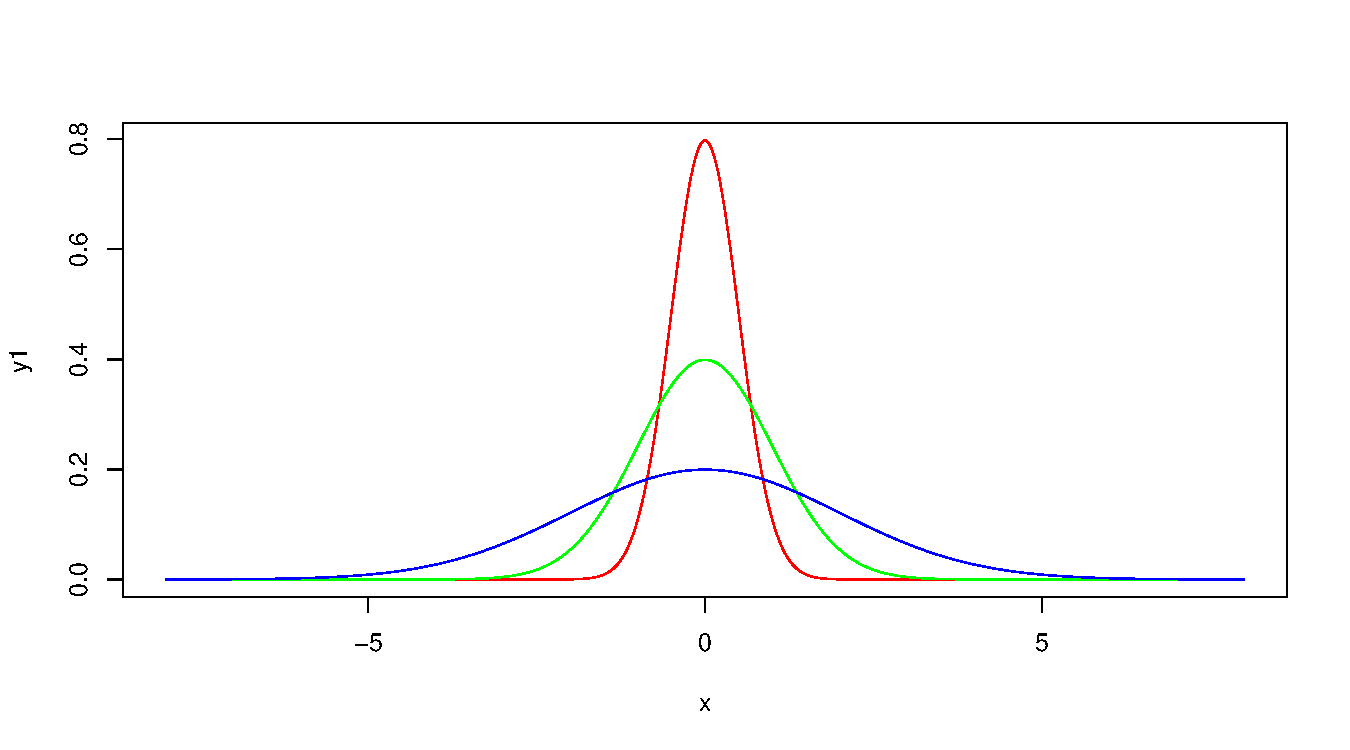
\includegraphics[scale=0.35]{pics/normplot.pdf}
\end{figure}



\end{frame}




\begin{frame}{Joint Probabilities}
\scriptsize{
\begin{itemize}
 \item The notion of probability function (mass or density) can be \textbf{extended} to more than one R.V.  
 \item Given a pair of discrete random variables $X$ and $Y$, define the joint mass function by $f(x,y) = \mathbb{P}(X = x $and$ Y = y)$ or $\mathbb{P}(X = x, Y = y)$.
 
 \item We write $f$ as $f_{X,Y}$ when we want to be more explicit.
 
 \item Example: Here is a bivariate distribution for two random variables $X$ and $Y$ each taking values 0 or 1:
 \begin{table}
\centering
 \begin{tabular}{c|cc|c}
& $Y=0$ & $Y=1$ & \\ \hline
$X=0$ & 1/9 & 2/9 & 1/3 \\
$X=1$ & 2/9 & 4/9 & 2/3 \\ \hline
& 1/3 & 2/3 & 1 \\
\end{tabular} 
\end{table} 
 
\item Thus, $f(1, 1) = \mathbb{P}(X = 1, Y = 1) = 4/9$. 
 


\end{itemize}

} 
\end{frame}

\begin{frame}{Joint Probabilities}
\scriptsize{

\begin{block}{Continuous Case}
In the continuous case, we call a function $f(x,y)$ a PDF for the random variables $(X, Y)$ if
\begin{enumerate}
 \item $f(x, y) \geq 0$ for all $(x, y)$,
 \item $\int_{-\infty}^{\infty} f(x,y)dxdy=1$ and,
 \item for any set $A \subset \mathbb{R}\times\mathbb{R}, \mathbb{P}((X,Y) \in A)=\int \int_{A}f(x,y)dxdy$. 
\end{enumerate}

\end{block}

In the discrete or continuous case we define the joint CDF
as $F_{X,Y} = \mathbb{P}(X \leq x, Y \leq y)$.

\begin{block}{Independent Random Variables}
\begin{itemize}
 \item Two random variables $X$ and $Y$ are independent if, for every $A$ and $B$, 
 \begin{displaymath}
\mathbb{P}(X \in A, Y \in B)=\mathbb{P}(X \in A)\times \mathbb{P}(Y \in B)                                                     \end{displaymath}
\item For the discrete case that means that $\mathbb{P}(X, Y) =\mathbb{P}(X)\times \mathbb{P}(Y)$ and for the continuous case we have that $f_{X,Y}(x, y) = f_{X}(x)\times f_{Y}(y)$ for all values $x$ and $y$.

\end{itemize}



\end{block}



} 
\end{frame}



\begin{frame}{Expectation}
\scriptsize{
\begin{itemize}
 \item Let $X$ be a R.V, we define its \textbf{expectation}, or \textbf{mean}, or \textbf{first-order moment} as:
  \begin{displaymath}
  \mathbb{E}(X) = \left\{ \begin{array}{rl}
  \sum_{x}(x\times f(x)) &\mbox{ If $X$ is discrete} \\
   \int_{-\infty}^{\infty}(x\times f(x))dx &\mbox{If $X$ is continuous}
       \end{array} \right.
  \end{displaymath}
\item The expectation is the weighted average of all the possible values that a random variable can take.
\item Think of $\mathbb{E}(X)$ as the average $\sum_{i=1}^{n}X_i/n$ of a large number of IID draws $X_1, \dots,X_n$. \footnote{This is  a theorem called the law of large numbers to be discussed next.}
\item For the case of tossing a coin twice with $X$ the number of heads:
 \begin{eqnarray*}
  \mathbb{E}(X) & = & (0 \times f(0)) + (1 \times f(1)) + (2 \times f(2)) \nonumber \\
       & = & (0 \times (1/4)) + (1 \times (1/2)) + (2 \times (1/4)) =1  \nonumber \\
 \end{eqnarray*}


\item Let the random variables $X_1, X_2, \dots , X_n$ and the constants $a_1, a_2, \dots, a_n$,
\begin{displaymath}
 \mathbb{E}\left(\sum_{i}a_i X_i \right) = \sum_{i} a_{i} \mathbb{E}(X_i)
\end{displaymath}
 


\end{itemize}
}

\end{frame}


\begin{frame}{Variance}
\scriptsize{
\begin{itemize}
 \item The variance measures the ``dispersion'' of a distribution.
 \item Lex $X$ be a R.V of mean $\mu$, we define the variance of $X$ denoted as $\sigma^2$, $\sigma^{2}_{X}$ or $\mathbb{V}(X)$ as:
  \begin{displaymath}
  \mathbb{V}(X) = \mathbb{E}(X - \mu)^2 =  \left\{ \begin{array}{rl}
  \sum_{i=1}^{n} f_{x}(x_{i})(x_{i} - \mu)^2 &\mbox{  If $X$ is discrete} \\
   \int (x- \mu)^{2}f_X(x)dx &\mbox{ If $X$ is continuous}
       \end{array} \right.
  \end{displaymath}
\item The \textbf{standard deviation} $\sigma$ is defined as $\sqrt{\mathbb{V}(X)}$ 
\end{itemize}

\begin{block}{Properties}
\begin{itemize}
\item $\mathbb{V}(X)=  \mathbb{E}(X^2)- \mathbb{E}(X)^2 =  \mathbb{E}(X^2)-\mu^2 $ 
\item If $a$ and $b$ are constants, then  $\mathbb{V}(aX+b)=a^2\mathbb{V}(X)$
\item If $X_1,\dots,X_n$ are independent and $a_1,\dots,a_n$ are constants, then
\begin{displaymath}
 \mathbb{V}\left(\sum_{i=1}^{n}a_i X_i \right) = \sum_{i=1}^{n} a_{i}^{2} \mathbb{V}(X_{i})
\end{displaymath}


\end{itemize}

 
\end{block}


}
\end{frame}

\begin{frame}{Expectation and Variance of Well-known Distributions}
 
\begin{figure}[h!]
	\centering
	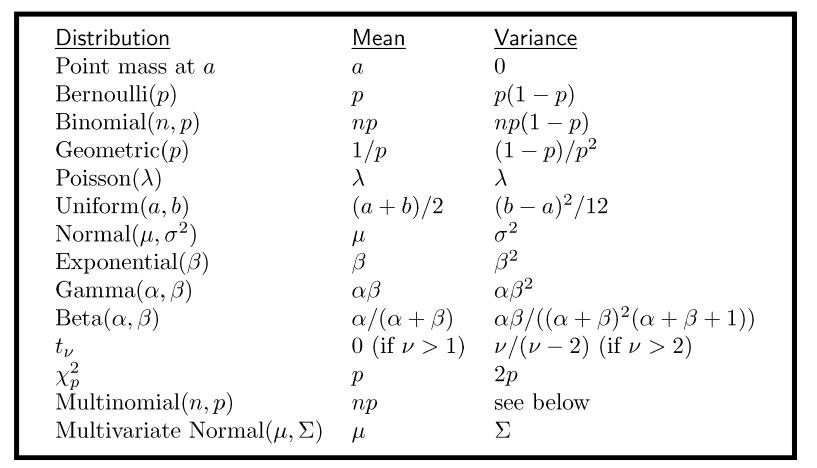
\includegraphics[scale=0.4]{pics/expectations.png}
\end{figure} 
 
\end{frame}



\begin{frame}{Law of the Large Numbers}
\scriptsize{
\begin{block}{Weak Form}
\begin{itemize}
\item This theorem says that the mean of a large sample is close to the mean of the distribution.
 \item Let $X_{1},X_{2},\dots X_{n}$ be IID random variables of mean $\mu$ and variance $\sigma^2$.
 \item The mean $\overline{X_{n}} =\frac{\sum_{i=1}^{n}X_{i}}{n}$ converges in probability to $\mu$, $\overline{X_{n}} \overset{P}{\rightarrow} \mu$   
 \item This is equivalent to saying that for all $\epsilon > 0$
 \begin{displaymath}
  \lim_{n\rightarrow \infty} \mathbb{P}(|\overline{X_{n}} - \mu| < \epsilon)=1
 \end{displaymath}
\item Then the distribution of  $\overline{X_{n}}$ more
concentrated around $\mu$ as $n$ grows.
\end{itemize}
\end{block}
\begin{block}{Example}
\begin{itemize}
 \item Let be the experiment of flipping a coin where the probability of heads is $p$.
 \item For a Bernoulli distributed R.V $\mathbb{E}(X)=p$.
 \item Let be $\overline{X_{n}}$ the fraction of heads after $n$ tosses.
 \item The law of large numbers tells us that  $\overline{X_{n}}$ converges in probability to $p$.
 \item This does not imply that  $\overline{X_{n}}$ is numerically equal to $p$.
 \item  But if $n$ in large enough, the distribution of $\overline{X_{n}}$ will be centered around $p$.
\end{itemize}

 
\end{block}



}
 
\end{frame}



\begin{frame}{The Law of Large Numbers}

\scriptsize{
\begin{itemize}
\item  Let's visualize executing the coin tossing experiment twice with $n=1,000$ and $p=0.5$ in the following plot.

\begin{figure}[h!]
	\centering
	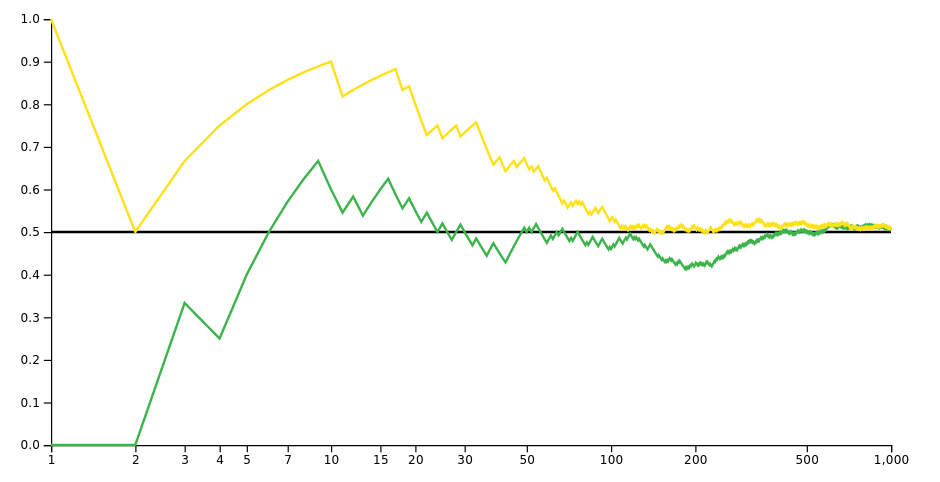
\includegraphics[scale=0.2]{pics/large_numbers.png}
\end{figure} 

\item On the x-axis we show the flip number and along the y-axis, we show the cumulative mean, or our average number of heads up to flip x. 

\item  Early on there is a lot of variation in mean scores. 
\item However, as you move towards 1,000 flips, the runs will converge towards the expected probability of 0.5. 
\item The more independent random events you have, the less variability there will be around the theoretically expected results.
 \end{itemize}

}
\end{frame}






\begin{frame}{Central Limit Theorem}
\scriptsize{
\begin{itemize}
 \item  While the law of large numbers tells us that  $\overline{X_{n}}$ approaches $\mu$ as $n$ grows.
 \item This is not sufficient to say anything about the distribution of  $\overline{X_{n}}$.
\end{itemize}

\begin{block}{Central Limit Theorem (CLT)}
\begin{itemize}
 \item Let $X_1, X_n$ be IID random variables of mean $\mu$ and variance $\sigma^2$.
 \item Let $\overline{X_{n}}=\frac{\sum_{i=1}^{n} X_i}{n}$
\begin{displaymath}
 Z_{n} \equiv \frac{\overline{X_{n}}-\mu}{\sqrt{\mathbb{V}(\overline{X_{n}})}}=\frac{\overline{X_{n}}-\mu}{\frac{\sigma}{\sqrt{n}}}  \rightsquigarrow Z
\end{displaymath}
where $Z\sim N(0,1)$
\item This is equivalent to:
\begin{displaymath}
 \lim_{n\rightarrow \infty} \mathbb{P}(Z_{n} \leq z) = \Phi(z) = \int_{-\infty}^{z}\frac{1}{\sqrt{2\pi}}e^{-x^2/2}dx
\end{displaymath}
\end{itemize}
\end{block}
\begin{itemize}
 \item The theorem allows us to approximate the distribution of $\overline{X_{n}}$ to a Gaussian distribution when $n$ is large. 
 \item Even if we do not know the distribution of $X_{i}$, we can approximate the distribution of its mean.
\end{itemize}



} 
\end{frame}

\begin{frame}{Central Limit Theorem (2)}
\scriptsize{
\begin{itemize}
 \item The previous example about the soccer field was a clear manifestation of the CLT.
 \item In that case we were summing up various independent random variables coming from a non-normal (Binomial) distribution.
 \item The CLT also holds for the sum of random variables, because the sum is just $\overline{X_{n}}$ multiplied by a constant.
\end{itemize}



\begin{block}{Alternative notations showing that $Z_{n}$ converges to a Normal}
\begin{eqnarray*}
  Z_n  &\approx &N(0,1)     \nonumber \\
  \overline{X_{n}} & \approx & N \left(\mu, \frac{\sigma^2}{n} \right)   \nonumber \\
  \overline{X_{n}}-\mu & \approx & N \left(0, \frac{\sigma^2}{n} \right)   \nonumber \\
  \sqrt{n}(\overline{X_{n}}-\mu) & \approx & N (0,\sigma^2) \nonumber \\
  \frac{\overline{X_{n}}-\mu}{\frac{\sigma}{\sqrt{n}}} & \approx & N (0,1) \nonumber \\
\end{eqnarray*}


\end{block}


 }
\end{frame}


\begin{frame}{ Why is the Central Limit Theorem Important?}
\scriptsize{
\begin{itemize}
 \item For experimentalists, the CLT is an extremely important concept. 
 \item For many practical questions, we cannot get measurements for an entire population of interest.
 \item So we have to select a sample from which to draw conclusions. 
 \item How can we be confident that the conclusions we draw about the sample generalize across the population? 
 \item The central limit theorem allows us to make claims about the distribution of our \textbf{sample means}. 
 \item This will be a fundamental idea for statistical inference.
\end{itemize}


 }
\end{frame}



\begin{frame}[fragile]{Example: Central Limit Theorem }
\scriptsize{
\begin{itemize}
 \item Suppose that the number of errors X of a computer program in a week follows a Poisson distribution with parameter $\lambda=5$.
 \item If $X \sim Poisson(\lambda)$, $\mathbb{E}(X)=\lambda$ and $\mathbb{V}(X)=\lambda$.
 \item This means that, on average, a computer program makes 5 errors in a week
 
 \item If we have 125 independent programs $X_{1},\dots,X_{125}$ we would like to approximate the probability that the average number of errors for all these programs during a week is less than 5.5:  $\mathbb{P}(\overline{X_{n}} < 5.5)$.



\end{itemize}






}
 
\end{frame}


\begin{frame}[fragile]{Example: Central Limit Theorem }
\scriptsize{
\begin{itemize}
 \item Using the CLT we have that:
 \begin{eqnarray*}
 \mathbb{P}(\overline{X_{n}} < 5.5) & = & \mathbb{P} \left( \frac{\overline{X_{n}}-\mu}{\frac{\sigma}{\sqrt{n}}} <  \frac{5.5 -\mu}{\frac{\sigma}{\sqrt{n}}}  \right) \nonumber \\ 
                                    & \approx & \mathbb{P}\left( Z < \frac{5.5 - 5}{\frac{\sqrt{5}}{\sqrt{125}}}  \right) = \mathbb{P}( Z < 2.5) =0.9938
\end{eqnarray*}

\item In R:

\end{itemize}

\begin{verbatim}
> n <- 125
> sigma <- sqrt(5)
> mu <-5
> pnorm(5.5,mean = 5,sd =sigma/sqrt(n))
[1] 0.9937903
> # alternatively
> pnorm(2.5)
[1] 0.9937903 
\end{verbatim}




}
 
\end{frame}

\begin{frame}{ Conclusions}
\scriptsize{
\begin{itemize}
 \item We have visited the main concepts of probability, the language uncertainty.
 \item Random variables, PDFs, PMFs, CDFs, are fundamental building blocks for statistical inference.
 \item The law of large numbers and the central limit theorem will allow us to make probabilistic statements about the population even if we only work with samples.
\end{itemize}


 }
\end{frame}



%%%%%%%%%%%%%%%%%%%%%%%%%%%
\begin{frame}[allowframebreaks]\scriptsize
\frametitle{References}
\bibliography{bio}
\bibliographystyle{apalike}
%\bibliographystyle{flexbib}
\end{frame}  










%%%%%%%%%%%%%%%%%%%%%%%%%%%

\end{document}
